%% his is file `elsarticle-template-1-num.tex',
%%
%% Copyright 2009 Elsevier Ltd
%%
%% This file is part of the 'Elsarticle Bundle'.
%% ---------------------------------------------
%%
%% It may be distributed under the conditions of the LaTeX Project Public
%% License, either version 1.2 of this license or (at your option) any
%% later version.  The latest version of this license is in
%%    http://www.latex-project.org/lppl.txt
%% and version 1.2 or later is part of all distributions of LaTeX
%% version 1999/12/01 or later.
%%
%% The list of all files belonging to the 'Elsarticle Bundle' is
%% given in the fil%e `manifest.txt'.
%%
%% Template article for Elsevier's document class `elsarticle' 
%% with numbered style bibliographic references
%%
%% $Id: elsarticle-template-1-num.tex 149 2009-10-08 05:01:15Z rishi $
%% $URL: http://lenova.river-valley.com/svn/elsbst/trunk/elsarticle-template-1-num.tex $
%%
%% \documentclass[preprint,12pt]{elsarticle}
%% Use the option review to obtain double line spacing
% \documentclass[preprint,review,12pt]{elsarticle}

%% Use the options 1p,twocolumn; 3p; 3p,twocolumn; 5p; or 5p,twocolumn
%% for a journal layout:
%% \documentclass[final,1p,times]{elsarticle}
%% \documentclass[final,1p,times,twocolumn]{elsarticle}
%% \documentclass[final,3p,times]{elsarticle}
\documentclass[final,3p,times,twocolumn]{elsarticle}
%% \documentclass[final,5p,times]{elsarticle}
%% \documentclass[final,5p,times,twocolumn]{elsarticle}

%% if you use PostScript figures in your article
%% use the graphics package for simple commands
%% \usepackage{graphics}
%% or use the graphicx package for more complicated commands
\usepackage{graphicx}
%% or use the epsfig package if you prefer to use the old commands
%% \usepackage{epsfig}

%% The amssymb package provides various useful mathematical symbols
\usepackage{mathtools}
\usepackage{color}
\usepackage{amssymb}
%% The amsthm package provides extended theorem environments
%% \usepackage{amsthm}

%% The lineno packages adds line numbers. Start line numbering with
%% \begin{linenumbers}, end it with \end{linenumbers}. Or switch it on
%% for the whole article with \linenumbers after \end{frontmatter}.
\usepackage{lineno}
%% natbib.sty is loaded by default. However, natbib options can be
%% provided with \biboptions{...} command. Following options are
%% valid:

%%   round  -  round parentheses are used (default)
%%   square -  square brackets are used   [option]
%%   curly  -  curly braces are used      {option}
%%   angle  -  angle brackets are used    <option>
%%   semicolon  -  multiple citations separated by semi-colon
%%   colon  - same as semicolon, an earlier confusion
%%   comma  -  separated by comma
%%   numbers-  selects numerical citations
%%   super  -  numerical citations as superscripts
%%   sort   -  sorts multiple citations according to order in ref. list
%%   sort&compress   -  like sort, but also compresses numerical citations
%%   compress - compresses without sorting
%%
\newcommand{\bsat}{b_{\mathrm{sat}}}
\newcommand{\qsat}{Q_{\mathrm{sat}}}
\newcommand{\xsat}{x_{\mathrm{sat}}}
\newcommand{\xunsat}{x_{\mathrm{unsat}}}
\newcommand{\xch}{x_{\mathrm{Chol}}}
\newcommand{\nbound}{b_{\mathrm{tot}}}
\newcommand{\lo}{l_{\mathrm{o}}}
\newcommand{\ldo}{l_{\mathrm{do}}}
\biboptions{sort&compress,super,numbers,comma,round}
%\biboptions{square,sort,comma,numbers}

\graphicspath{{../Images/}}
\journal{BBA}
\newcommand{\nachr}{nAChR}
\newcommand{\grace}[1]{\textcolor{blue}{#1}}
\newcommand{\graceforgrace}[1]{\textcolor{green}{#1}}
\newcommand{\liam}[1]{\textcolor{red}{#1}}
\newcommand{\del}[1]{\textcolor{cyan}{#1}}

\begin{document}

\begin{frontmatter}

%% Title, authors and addresses

%% use the tnoteref command within \title for footnotes;
%% use the tnotetext command for the associated footnote;
%% use the fnref command within \author or \address for footnotes;
%% use the fntext command for the associated footnote;
%% use the corref command within \author for corresponding author footnotes;
%% use the cortext command for the associated footnote;
%% use the ead command for the email address,
%% and the form \ead[url] for the home page:
%%
%% \title{Title\tnoteref{label1}}
%% \tnotetext[label1]{}
%% \author{Name\corref{cor1}\fnref{label2}}
%% \ead{email address}
%% \ead[url]{home page}
%% \fntext[label2]{}
%% \cortext[cor1]{}
%% \address{Address\fnref{label3}}
%% \fntext[label3]{}

\title{Boundary lipids of the nicotinic acetylcholine receptor: spontaneous partitioning via coarse-grained molecular dynamics simulation} 
%% use optional labels to link authors explicitly to addresses:
%% \author[label1,label2]{<author name>}
%% \address[label1]{<address>}
%% \address[label2]{<address>}

\author[ccib]{L. Sharp} 
\author[ccib,wasu]{R. Salari}
\author[ccib,physics]{G. Brannigan}
%GB: set your affiliation as CCIB & set mine as CCIB and physics dept 
\address[ccib]{Center for Computational and Integrative Biology, Rutgers University-Camden, Camden, NJ}
\address[wasu]{Now at Washington University School of Medicine in St Louis}
\address[physics]{Department of Physics, Rutgers University-Camden, Camden, NJ}

\begin{abstract}
%% Text of abstract
Reconstituted nicotinic acetylcholine receptors (nAChR) exhibit significant gain-of-function upon addition of cholesterol to reconstitution mixtures, and cholesterol affects organization of nAChRs within domain-forming membranes, but whether \nachr~partitions to cholesterol-rich liquid-ordered (``raft``) domains or cholesterol-poor liquid-disordered domains is unknown.  
%The functional sensitivity of nicotinic acetylcholine receptors (nAChR) to membrane lipids is well-established, and it has been demonstrated numerous times that adding at least 10-15\% cholesterol can restore nAChR native function in model phosphatidylcholine model membranes.  Along with images of nAChR clustering, it has been hypothesized that nAChRs partition to cholesterol rich liquid-ordered (``raft'') domains within membranes, although this has not been directly observed.  
We use coarse-grained molecular dynamics (MD) simulations to observe spontaneous interactions of cholesterol, saturated lipids, and polyunsaturated lipids with \nachr s. 
% in binary cholesterol-containing model membranes as well as ternary domain-forming membranes inspired by native nAChR membranes, which include high levels of $n-3$ polyunsaturated fatty acids (PUFAs), saturated fatty acids, and cholesterol. 
In binary Dipalmitoylphosphatidylcholine:Cholesterol (DPPC:CHOL) mixtures, both CHOL and DPPC acyl chains were observed spontaneously entering deep ``non-annular'' cavities in the \nachr~TMD, particularly at the subunit interface and the $\beta$ subunit center, facilited by the low amino acid density in the cryo-EM structure of nAChR in a native membrane.  Cholesterol was highly enriched in the annulus around the TMD, but this was a short range effect that extended over (at most) 5-10\AA. 
%The two PUFAs chosen for these simulations were Docosahexaenoic acid and Linoleic acid.
In ternary mixtures containing polyunsaturated fatty acids (PUFAs), the presence of a single receptor did not significantly affect the likelihood of domain formation, and nAChR partitioned to the cholesterol-poor liquid-disordered domain whenever one was present. This was independent of whether the $\ldo$ domain lipids had PC or PE headgroups, but saturated lipids with PE headgroups were less depleted from the boundary than those with PC headgroups. % frequently near the boundary of the liquid-ordered domain. 
%Analysis of boundary lipid composition indicates enrichment of PUFA chains, particularly $n-3$ chains (tested here with Docosahexaenoic Acid, DHA), and to a lesser extent, $n-6$ chains (represented here with Linoleic acid,\graceforgrace{need to be consistent with lipid} LoA), regardless of whether the headgroup for the PUFA containing lipid is PC or PE, while Saturated lipids are moderately less likely to be depleted from the \nachr~boundary with a PE headgroup than a PC headgroup.  % a  confirms nAChR boundary lipids are enriched in PUFAs. 
%$\alpha$ subunits, however, indicate a preference for cholesterol rich domains, potentially facilitating partitioning near the interface. 
Enrichment of unsaturated phospholipids among boundary lipids was positively correlated with their propensity for demixing from cholesterol-rich phases. Long $n-3$ chains (tested here with Docosahexaenoic Acid, DHA) were highly enriched in annular and non-annular embedded sites, partially displacing cholesterol and completely displacing DPPC, and occupying sites even deeper within the bundle. Shorter $n-6$ chains (Linoleic acid, LA) were far less effective at displacing cholesterol from non-annular sites.   % , with PUFA acyl chains preferred over cholesterol in most sites.   %  while beta subunits show preference for PUFAs. Lastly, analysis shows PUFAs and cholesterol binding non-annularly nAChR. 

\end{abstract}

\begin{keyword}
Polyunsaturated Fatty Acids (PUFA) \sep Docosahexaenoic acid (DHA) \sep cholesterol \sep nicotinic acetylcholine receptor \sep nAChR partitioning \sep liquid order ($l_o$) \sep liquid disorder ($l_{do}$) \sep lipid-protein interactions \sep lipid rafts
%% keywords here, in the form: keyword \sep keyword

%% MSC codes here, in the form: \MSC code \sep code
%% or \MSC[2008] code \sep code (2000 is the default)

\end{keyword}

\end{frontmatter}
%%
%% Start line numbering here if you want
%%
\linenumbers
%% main text
\section{Introduction}
\label{S:1}
The nicotinic acetylcholine receptor (nAChR) is an excitatory pentameric ligand gated ion channel (pLGIC) commonly found in the post synaptic membrane, neuromuscular junction (NMJ) \cite{Breckenridge_Adult_1973,Cotman_Lipid_1969} and the \textit{Torpedo} electric organ \cite{8DAAC844-CF26-B5A6-FE56-AEE1F681B8A3,Quesada_Uncovering_2016} . nAChR is found at concentrations around $10^4$ $\mu m^{-2}$ within the NMJ membrane \cite{Breckenrldge1972}. 

The pLGIC super family has been shown to play roles in cognition \cite{Walstab2010}, inflammation \cite{Patel2017,Yocum2017,Cornelison2016}, addiction \cite{Cornelison2016}, chronic pain \cite{Xiong2012} and numerous diseases including: Alzheimer's Disease, spinal muscular atrophy, and neurological autoimmune disease \cite{MartinRuiz_4_1999, Arnold_Reduced_2004,Lennon_Immunization_2003,Papke_The_2012,Picciotto_Neuroprotection_2008}. nAChR plays a major role in excitation of the central and peripheral nervous system and binds agonists such as nicotine, acetylcholine and general anesthetics in multiple sites \cite{Bondarenko_NMR_2013,Jayakar_Identification_2013,LeBard_General_2012,Brannigan_Multiple_2010}.

nAChR is highly lipid sensitive and is functionally dependent on cholesterol and anionic lipids when reconstituted into a membrane \cite{Fong_Correlation_1986,Sunshine_Lipid_1992,Hamouda_Assessing_2006,Butler_FTIR_1993,Bhushan_Correlation_1993,Fong_Stabilization_1987,Bednarczyk_Transmembrane_2002,Corrie_Lipid_2002}. Lacking native-like concentrations of cholesterol or an abundance of anionic lipids in reconstituted membranes does not inhibit ligand-nAChR binding, but prevents gating and conformational changes \cite{Baenziger2015,Carswell_Role_2015,Calimet2013}, impeding ion flux through the pore \cite{Fong_Correlation_1986,Sunshine_Lipid_1992,Hamouda_Assessing_2006,Butler_FTIR_1993,Bhushan_Correlation_1993,Fong_Stabilization_1987,Bednarczyk_Transmembrane_2002,Corrie_Lipid_2002,Cheng_Anionic_2009}. Previous research suggests cholesterol may be bound within the inter- and intra-subunits of the transmembrane domain (TMD) \cite{Brannigan_Embedded_2008}; and cholesterol has been hypothesized and recently found bound within the $\gamma$-Aminobutyric acid receptors (GABAARs) TMD \cite{Hnin_A_2014,Laverty2017}. 

nAChR's native membranes (\textit{Torpedo}, synaptic)\cite{Breckenridge_Adult_1973,Cotman_Lipid_1969,8DAAC844-CF26-B5A6-FE56-AEE1F681B8A3,Quesada_Uncovering_2016}, are enriched in phosphoethanolomine (PE) and polyunsaturated fatty acids (PUFAs) when compared oocyte\cite{Hill_Isolation_2005}, and a generalized mammalian cell \cite{Inglfsson_Lipid_2014}. Unsaturated lipids are likely to form domains as unsaturated acyl chain's disorder prevents unsaturated lipids from easily mixing with the rigid saturated-, sphingolipids and cholesterol \cite{Feller_Acyl_2008,Yeagle2016115}; forming domains depleted in cholesterol, labeled liquid disordered ($l_{do}$) domains. Domain formation has been studied both experimentally and computationally in model membranes \cite{Lingwood_Lipid_2010,Kaiser_Order_2009,Ma_n_2004,Inglfsson_Lipid_2014,Risselada_The_2008}, showing de-mixing of lipids with saturated fatty acids and unsaturated fatty acids \cite{Levental_Polyunsaturated_2016,Lor2015}.

%Monounsaturated fatty acids contain a single double bond, while PUFA's contain two or more double bonds through their acyl chain. These double bonds make unsaturated lipids both disordered and highly flexible \cite{Lingwood_Lipid_2010,Pato_Role_2008,Risselada_The_2008,Schley_2007,Rawicz_Effect_2000}. 


%PE (a zwitterionic head group) is one of two major head groups, the other being phosphocholine (PC). nAChR-lipid studies using model membranes with zwitterionic head groups have not included PUFAs, instead favoring saturated and monounsaturated fatty acids. %need proper refs

nAChR's functional dependency on cholesterol has suggested that nAChR partitions into ordered cholesterol enriched domains \cite{Bermdez_Partition_2010,Perillo_Transbilayer_2016,Pato_Role_2008,Fong_Correlation_1986,Sunshine_Lipid_1992}, liquid ordered ($l_o$) domains. Bermdez et al \cite{Bermdez_Partition_2010}, showed nAChR to partitioned equally into $l_o$ and $l_{do}$ domains in model membranes of Chol:POPC:SM 1:1:1. Expanding on \cite{Bermdez_Partition_2010}, Perillo et al \cite{Perillo_Transbilayer_2016} showed using the previous composition but inducing asymmetrical membrane compositions, promoted nAChR to partition into the $l_o$ domain.% These results may represent nAChR sitting at an interface instead of in a $l_{do}$ domain. %Research predicting nAChR partitioning into  $l_o$ phase have used model membranes composed of cholesterol, lipids with saturated acyl chains, and lipids with anionic head groups (such as  Palmitoyloleoylphosphatidylcholine (POPC) and  Palmitoyloleoylphosphatidic acid  (POPA)). 

Through coarse grained molecular dynamics simulations, we have analyzed nAChR-lipid interaction within quasi-native membrane using the cryo-EM nAChR structure derived by Unwin in 2005 \cite{Unwin_Refined_2005}. The coarse grained model allows for significantly larger systems to be constructed using atomistic models. Running simulations over $\mu s$ allows systems to approach equilibrium, showing domain formation and protein partitioning. 

We use the PUFAs Docosahexaenoic acid (22:6 $n-3$) (DHA) and Linoleic acid (18:2 $n-6$) (LA). Nearly all the $n-3$ PUFAs in both synaptic and \textit{Torpedo}'s electric organ have been determined to be DHA \cite{Breckenridge_Adult_1973,Cotman_Lipid_1969,8DAAC844-CF26-B5A6-FE56-AEE1F681B8A3,Quesada_Uncovering_2016}. LA was a useful test fatty acid; Risselada et al \cite{Risselada_The_2008} showed it a usable PUFA for domain formation using Martini \cite{martini}.

Our simulations show embedded nAChR consistently partitions into the  $l_{do}$ phase. This research explores nAChR's partitioning behavior, boundary lipid affinity, and deep non-annular lipid-protein interactions termed ''embedding'' within domain forming membranes. It is our understanding this is the first study applying coarse grained molecular dynamics to nAChR in a membrane containing the most prominent native PUFA, DHA.
\section{Methods}
\label{S:2}
% !TEX root = main.tex
\subsection{System Composition}

All simulations reported here used the coarse-grained MARTINI 2.2\cite{martini} topology and forcefield.%, which was necessary for allowing sufficient lipid diffusion to equilibrate mixed membranes.  
~nAChR coordinates were based on a cryo-EM structure of the $\alpha{\beta}\gamma\delta$ muscle-type receptor in native torpedo membrane (PDB 2BG9\cite{Unwin_Refined_2005}). This is a medium resolution structure (4\AA) and was further coarse-grained using the martinize.py script; medium resolution is sufficient for use in coarse-grained simulation, and the native lipid environment of the proteins used to construct 2BG9 is critical for the present study. The secondary, tertiary and quaternary structure in 2BG9 was preserved via soft backbone restraints during simulation as described below, so any inaccuracies in local residue-residue interactions would not cause instability in the global conformation.  

Coarse-grained membranes were built using the Martini script insane.py, which was also used to embed the coarse-grained \nachr~within the membrane. The insane.py script randomly places lipids throughout the inter- and extra-cellular leaflets, and each simulation presented in this manuscript was built separately.  Binary mixed membranes were composed of one saturated lipid species (Dipalmitoylphosphatidylcholine-DPPC or Dipalmitoylphosphatidylethanolamine-DPPE) and cholesterol (CHOL), while ternary mixed membranes also included either two $n-6$ PUFA acyl chains : Dilinoleoylphosphatidylcholine (DLiPC) or Dilinoleoylphosphatidylethanolamine (DLiPE) or two $n-3$ PUFA acyl chains : Didocosahexaenoylphosphatidylethanolamine (DHA-PE) or Didocosahexaenoylphosphatidylcholine (DHA-PC). DHA-PC is not distributed with the MARTINI lipidome, but was constructed in-house using MARTINI DHA tails and PC headgroups). Multiple box sizes were used depending on the goal;  ``small'' boxes were between $22x22x20$ nm$^3$ and $25x25x25$ nm$^3$, with about {$\sim$ 1400} total lipids and {$\sim$ 80000} total beads, and were used primarily to investigate composition trends, ``large'' boxes were about $45x45x40$ nm$^3$ with about {$\sim$ 8,300} total lipids and {$\sim$ 820,000} total beads, and were used primarily to investigate subunit specificity and long-range sorting, and ``very large'' boxes were $\sim$ 75x75x40~nm$^3$ with about {$\sim$ 19,000} total lipids and {$\sim$ 1.8 million} total beads, and were used to verify that partitioning in the $\ldo$ phase did not reflect finite size effects.  

%The saturated lipids used are Dipalmitoylphosphatidylcholine (DPPC), Dipalmitoylphosphatidylethanolamine(DPPE). The PUFAs used were Didocosahexaenoylphosphatidylethanolamine (DHA-PE), Didocosahexaenoylphosphatidylcholine (DHA-PC), Dilinoleoylphosphatidylcholine (DLiPC), and Dilinoleoylphosphatidylethanolamine (DLiPE). Cholesterol (Chol) was the only sterol used. 
%The lipids used are Dipalmitoylphosphatidylcholine (DPPC), Dipalmitoylphosphatidylethanolamine(DPPE), Didocosahexaenoylphosphatidylethanolamine (DHA-PE), Didocosahexaenoylphosphatidylcholine (DHA-PC), Dilinoleoylphosphatidylcholine (DLiPC), Dilinoleoylphosphatidylethanolamine (DLiPE) and cholesterol (Chol).

\subsection{Simulations}


Molecular dynamics simulations were carried out using GROMACS\cite{grom}; small boxes used GROMACS 5.0.6 and large boxes used  GROMACS 5.1.2 or 5.1.4. All systems were run using van der Waals (vdW) and Electrostatics in shifted form with a dielectric constant of $\epsilon_r$=15. vdW cutoff lengths were between 0.9 and 1.2 nm, with electrostatic cutoff length at 1.2 nm.

Energy minimization was performed over 10000 to 21000 steps.  Molecular dynamics were run using a time step of 25~fs, as recommended by MARTINI, for 2 $\mu$s for {small membranes,and 10 $\mu$s for large and very large membranes}. Simulations were conducted in the isothermal-isobaric (NPT) ensemble, by using a Berendsen thermostat set to 323 K with temperature coupling constant set to  1 ps, as well as isotropic pressure coupling with compressibility set to $3\times 10^{-5}$ bar$^{-1}$ and a pressure coupling constant set to 3.0 ps. %All systems were run using van der Waals (vdW) and Electrostatics in shifted form with a dielectric constant of $\epsilon_r=15$. vdW cutoff lengths were between 0.9 and 1.2 nm, with electrostatic cutoff length at 1.2 nm.

%However most energy minimizations finished within $\sim$ 1700 to 3000 steps. Molecular dynamics were run using a time step 0.025 $ps$ for 2 $\mu$s. Simulations used  NPT ensembles. We used Berendsen thermostat with an isotropic pressure couple. The reference temperature was set to 323 Kelvin with temperature coupling constant set to  1 $ps$. The system's compressibility is set to $3e^{-5}$ $bar^{-1}$ and a pressure coupling constant of 3.0 $ps$. 
%\liam{In the case of systems at $45x45x40$ $nm^3$, Martini 2.2 and Gromacs 5.1.2 and 5.1.4 were used. Parameters remain the same, however energy minimization was carried out to $\sim$ 21000 steps, and 12.5 $ns$ of NPT equilibration were performed before $\sim 4.5-5 \mu s$ simulation was performed.}

Secondary structures restraints consistent with MARTINI recommendations were constructed by the martinize.py \cite{martini} script {and} imposed by Gromacs\cite{grom}. Protein conformation was maintained in small systems via harmonic restraint (with a spring constant of 1000 kJ$\cdot$ mol$^{-1}$) on the position of backbone beads. \nachr~conformation in large systems was preserved via harmonic bonds between backbone beads separated by less than 0.5 nm. Based on Martini's \cite{martini} ElNeDyn algorithm \cite{Periole_Combining_2009} with a harmonic constant of 900 kJ$\cdot$ mol$^{-1}$.  These restraints limited the root-mean-squared-displacement (RMSD) of the backbone to less than 2.5 \r{A} throughout the simulation.  

The minimum equilibration time depended on the system size. Small systems typically began domain formation by 500 ns, with domains fully formed by 1000 ns. Large systems and very large simulations required about 5$\mu$s of equilibration for stabilization of $M_{DHA,DHA}$.

\subsection{Analysis}

Extent of domain formation within the membrane was tracked by 
    \begin{equation}
    \begin{aligned}
      M_{A, B} = \frac{\langle n_{A,B} \rangle} {6x_{B}} -1 
    \end{aligned}
    \label{eq:M}
  \end{equation}
 where $n_{A,B}$ is the number of type B molecules among the 6 nearest neighbors for a given type A molecule, and the average is over time and all molecules of type $A$. For a random mixture, $\langle n_{A,B} \rangle = 6x_{B}$, where $x_{B}$ is the fraction of overall bulk lipids that are of type B. ${M_{A,B}~0}$ indicates random mixing while ${M_{A,B}>0}$  and ${M_{A,B}<0}$ indicate demixing and excessive mixing respectively.  

%	$M_{a,b}$ compares measured and expected mixing, where $a$ and $b$ represent a reference and a local lipid species respectively, equation \ref{eq:M}. 
%    \begin{equation}
%    \begin{aligned}
%      M_{a,b} = \frac{\langle \eta_{a,b} \rangle} {\langle \eta_{a,b} \rangle_{rand}} - 1
%    \end{aligned}
%    \label{eq:M}
%  \end{equation}
%  We define $\eta_{a,b}$ as the percentage of lipid species $b$ in contact with lipid species $a$. $M_{a,b}$ is subtracted by one to include all points.

Extent of receptor partitioning within the $\lo$ or $\ldo$ domain was tracked by counting the number $\bsat$ of saturated boundary lipids and comparing with the expectation for a random mixture, via the order parameter $\qsat$:
  \begin{equation}
    \begin{aligned}
      \qsat\equiv \frac{1}{\xsat}\left\langle\frac{  \bsat }{\nbound }\right\rangle-1,\\
    \end{aligned}
    \label{eq:Q}
  \end{equation}
  where $\nbound$ is the total number of lipids in the boundary region and $\xsat$ is the fraction of overall bulk lipids that are saturated phospholipids. $\qsat <0$ indicates depletion of saturated lipids among boundary lipids, as expected for partitioning into an $\ldo$ phase, while $\qsat>0$ indicates enrichment and likely partitioning into an $\lo$ phase. Each frame, $\nbound$ and $\bsat$ were calculated by counting the number of total and saturated lipids, respectively, for which the phosphate bead fell within a distance of 10~\AA~ to 35~\AA~ from the M2 helices, projected onto the membrane plane. 
  
  Two-dimensional density distribution of the beads within a given lipid species $B$ around the protein was calculated on a polar grid: %$\rho_a$ (\r{A}$^{-2}$) is the density of lipid $a$ within a given bin equations \ref{eq:R}.
  \begin{equation}
    \begin{aligned}
      \rho_{B}(r_i,\theta_j)= \frac{\left\langle n_{B}(r_i,\theta_j) \right\rangle}{r_i \Delta{r}\Delta{\theta}} \\        
    \end{aligned}
    \label{eq:R}
  \end{equation}
  where  $r_i = i \Delta{r}$ is the projected distance of the bin center from the protein center, $\theta_j = j \Delta{\theta}$ is the polar angle associated with bin j,  $\Delta{r}$= 10\AA~ and  $\Delta{\theta} = \frac{\pi}{15}$ radians are the bin widths in the radial and angular direction respectively, and $\left\langle n_{B}(r_i,\theta_j) \right\rangle$ is the time-averaged number of beads of lipid species $B$ found within the bin centered around radius $r_{i}$ and polar angle $\theta_{j}$.  In order to determine enrichment or depletion, the normalized density $ \tilde{\rho}_{B}(r_i,\theta_j)$ is calculated by dividing by the approximate expected density of beads of lipid type B in a random mixture, $x_{B}s_{B}~N_{L}/\langle L^{2}\rangle$, where $s_{B}$ is the number of beads in one lipid of species B, $N_{L}$ is the total number of lipids in the system, and $\langle L^{2}\rangle$ is the average projected box area: 
  \begin{equation}
    \begin{aligned}
  \tilde{\rho}_{B}(r_i,\theta_j)=\frac{ \rho_{B}(r_i,\theta_j)}{x_{B}s_{B}~N_{L}/\langle L^{2}\rangle} \\        
    \end{aligned}
    \label{eq:Rt}
  \end{equation}
  This expression is approximate because it does not correct for the protein footprint or any undulation-induced deviations of the membrane area.  The associated corrections are small compared to the membrane area and would shift the expected density for all species equally, without affecting the comparisons we perform here.   
   %However, as a result of smaller boxes, protein-protein interaction across the periodic boundary resulted in a ''pinwheeling'' effect. 

   %To compensate this, $\rho$ was adjusted by the thickness of the membrane
   %\begin{equation}
   % \begin{aligned}
   %   \tilde{\rho}_{B,i}=\rho_{B,i}\left\langle\frac{1}{\til%de{z}_{i}}\right\rangle \\        
   % \end{aligned}
   % \label{eq:Til}
  %\end{equation}
 %, \liam{$\tilde{z}_{i}$ is the thickness of a membrane per total number of lipids in a given bin}. %In the case of Cartesian bins, $A = \Delta{x} \Delta{y}$ where 
 
 %\liam{Regardless of the pinwheeling effect, 
  
\section{Results}
\label{S:3}
% !TEX root = main.tex
\begin{figure*}[h!]
	\center
	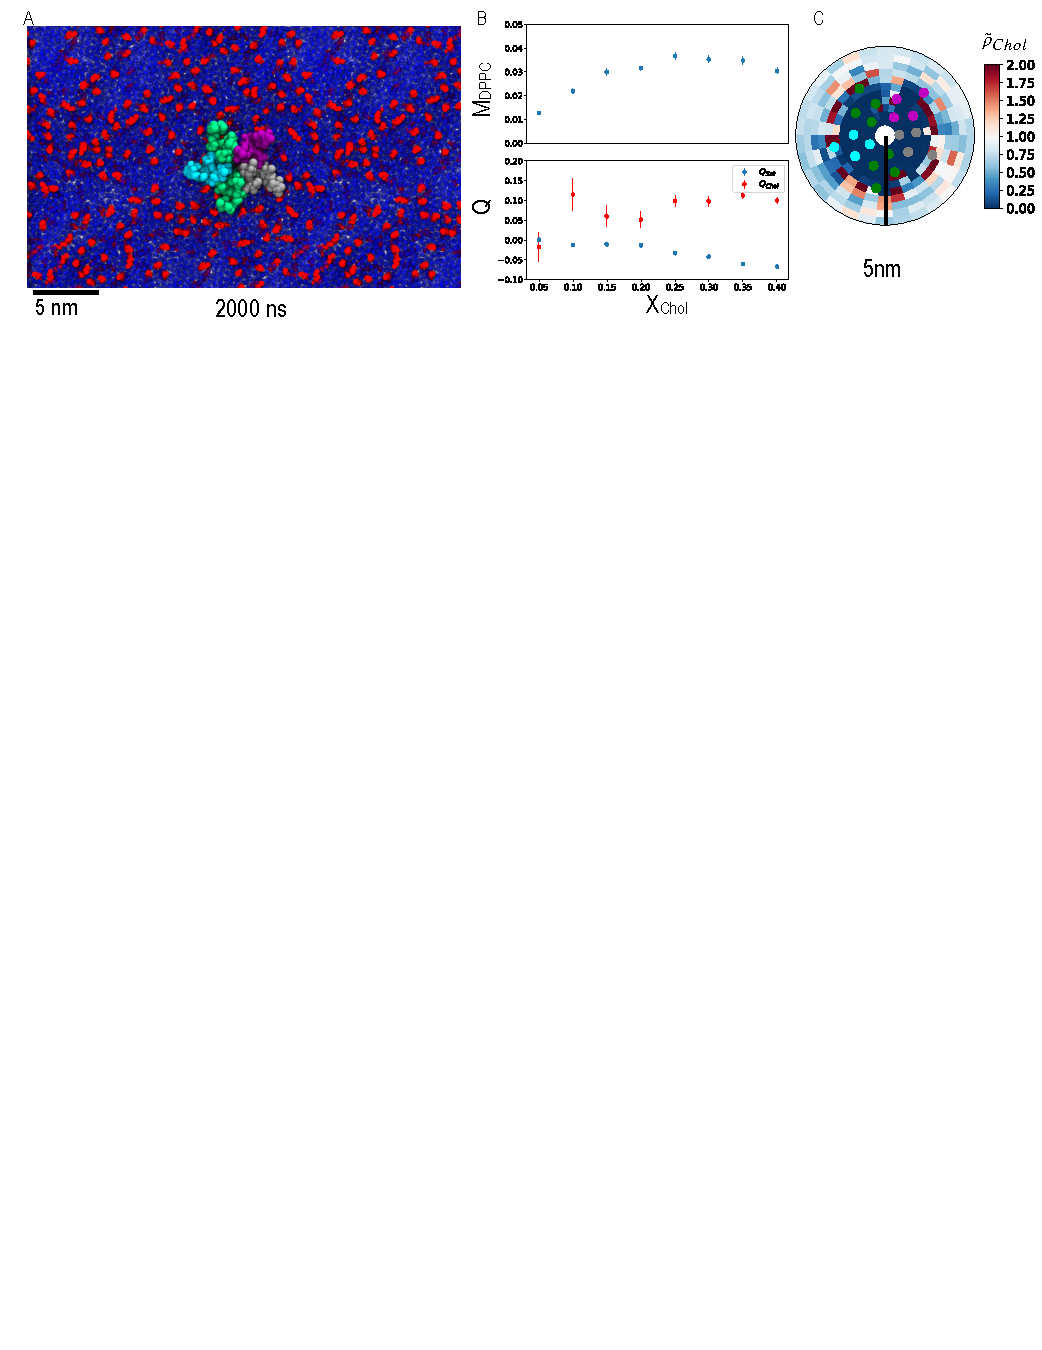
\includegraphics[width=\linewidth]{DPPC_Only.pdf}
	\caption{nAChR boundary lipids in binary mixtures of DPPC and CHOL. A: Representative frame from a simulated trajectory of a single nAChR embedded in a small membrane, colored by subunit ($\alpha$:green, $\beta$:purple, $\delta$:gray, $\gamma$:cyan) in a 4:1 DPPC (blue):Chol (red) mixture.  B: Extent of demixing ($M_{DPPC,DPPC}$ defined in Eq. \ref{eq:M}) and depletion of saturated lipids from the boundary ($\qsat$ defined in Eq.\ref{eq:Q}) in small binary membranes. In this binary system, cholesterol depletion/enrichment is directly related to the saturated lipid depletion/enrichment: $Q_\mathrm{chol}=-x_{\mathrm{sat}} \qsat/\xch$.  Error bars represent standard error for a blocking average over 50 ns. C: Average normalized density (Eq. \ref{eq:Rt}) of cholesterol for the system in A. Plot shown is identical to Figure \ref{fig:sorting} in ``Chol'' row, ``None'' column, but has been cropped and zoomed around the protein center.\grace{Update previous sentence upon inclusion of new figure}}
	\label{fig:binary}
\end{figure*} 
\subsection {Spontaneous association with cholesterol in binary membranes} \label{binary}

%We previously proposed that cholesterol could be embedded within intersubunit and intrasubunit sites of \nachr\cite{Brannigan_Embedded_2008} or intersubunit sites of the GABA(A) receptor\cite{Brannigan_Embedded_2008}.  It was recently found in \cite{Laverty2017}, to embed within the inter- and intra-subunits of nAChR and other pLGICs. Docking has been used in previous computational research to determine optimal cholesterol binding domains \cite{Hnin_A_2014,Brannigan_Embedded_2008}, but coarse grained systems have shown to be a novel method to simulate non-annular lipid binding without the need to dock lipids within proteins. \liam{Figure \ref{fig:binary} measures an absence of embedded DPPC but an enrichment of cholesterol embedding throughout the protein.}
Lipid sorting was characterized for \nachr s in binary DPPC:CHOL membranes (Figure \ref{fig:binary}A)  using several metrics. 
Non-random lipid mixing (including domain formation) was quantified using the self-association metric $M_{A,A}$ as defined in Equation \ref{eq:M}. %; this quantity reflects degree of self-association of DHA-containing and LA-containing lipids respectively.  %enrichment of lipid species $B$ among the nearest neighbors of lipid species $A$ , with values close to 0 indicating random mixing, and positive and negative values indicating enrichment or depletion of species $B$ around species $A$, respectively. $M_{A,B}>> 0$ indicates substantial demixing and domain formation.  
As expected, in simulated binary membranes containing only DPPC and 0-40\% cholesterol, minimal demixing was observed, with values of $M_{DPPC,DPPC}$ (Fig \ref{fig:binary}B) rising slightly for higher cholesterol concentrations but remaining persistently below 0.05.  %Similar values were observed for $M_{CHOL,CHOL}$.

Depletion of saturated lipids among \nachr~boundary lipids (relative to those expected for a random mixture) was quantified using the metric $\qsat$ defined in equation \ref{eq:Q}. Negative and positive values of $\qsat$ reflect depletion or enrichment of saturated lipids in the \nachr~boundary, respectively. In binary systems containing cholesterol and saturated lipids, depletion of saturated lipids corresponds directly to enrichment of cholesterol: $Q_{chol} = -\qsat x_{sat}/\xch$. %, respectively, while values of $\qsat$ approaching 1 or -1 indicates partitioning within a well-defined $\lo$ or $\ldo$ phase, respectively.

In binary DPPC:CHOL mixtures, $\qsat$ was very slightly negative for $\xch < 20\%$, but decreased steadily for higher concentrations. This trend indicates some depletion of DPPC (and enrichment of cholesterol) among \nachr~ boundary lipids (Figure \ref{fig:binary}B).  Typically, between 10 and 20\% cholesterol has been required in reconstitution mixtures to restore native function  \cite{Fong_Correlation_1986,Dalziel1980,Criado1982}  and a phase transition at about 20\% cholesterol in binary DPPC:CHOL model membranes is indicated by differential scanning calorimetry.\cite{Marsh2010} 

Spontaneous binding of cholesterol to non-annular or ``embedded'' sites, similar to what we previously proposed\cite{Brannigan_Embedded_2008}, was observed in these CG-simulations, and penetration of the TMD bundle by DPPC acyl chains was also observed at lower cholesterol concentrations (Fig \ref{fig:binary}A).  Distribution of density for embedded lipids is further discussed in Section 3.4.  %deep binding of lipids was much more common in the subunit interfaces, particularly $\alpha/\beta$ and $\delta/\alpha$, than in the subunit center (Figure \ref{fig:sorting})\liam{. A}lthough DPPC partitioned extensively to the relatively large cavity in the center of the $\beta$ subunit.  

Annular cholesterol (enrichment of cholesterol at the protein-lipid interface), is visible for the binary systems via a ring of high (red) cholesterol density just around the protein in Figure \ref{fig:binary}C. Enrichment of cholesterol near the protein is highly localized with a ring that is less than 5\AA~wide. This is in general agreement with evidence for annular cholesterol in randomly-mixed binary membranes. \cite{Barrantes2010}

%at low concentrations of cholesterol, \liam{it is} almost entirely within ``embedded'' or non-annular \liam{region of the protein} (Figure \ref{fig:binary}C) as predicted in \cite{Brannigan_Embedded_2008}.
%Intriguingly, all simulations consistently yielded four general regions of differential embedded cholesterol density : a high density region ($\alpha_{\gamma}/\gamma$ interface and center of the $\alpha$ subunit), a low/background density region ($\beta/\alpha_{\gamma}$ interface and center of $\beta$ subunit) on the opposite face of the TMD, and two regions of intermediate density that separated them.  In the absence of nAChR, DPPC/CHOL lipid bilayers are randomly mixed, so this result indicates an intrinsic cholesterol amphipathy.  

%At higher concentrations of cholesterol, cholesterol was also enriched in ``annular'' sites, particularly at the high affinity and low affinity face of the TMD.  This enrichment actually extended many lipidation shells off the high affinity face, indicating nAChR was not just sorting lipids, but even inducing organization of the membrane. Enrichment far from the TMD is expected to be particularly sensitive to finite size effects, although there is no clear reason for why these effects would consistently have a dependence on protein orientation.  
% , and two intermediate density regions (1: $\gamma-/\alpha+$ face and subunit center of both subunits and 2: ) and $\delta-/\alpha+$ faces, and nearly background density on the $\alpha-/\beta+$ face.  As a result, the protein overall 


\subsection {Domains formed in PUFA-containing ternary membranes are not affected by introduction of an \nachr } \label{Demix}
	\begin{figure}[h!]
		\center
		\includegraphics[width=1\linewidth]{Fig2.pdf}
		\caption{Quantitative analysis of bulk membrane mixing and nAChR boundary lipid composition across small membranes containing DPPC, Cholesterol, and either dDHA-PE or dLiPC. Shaded contours were constructed based on 40 individual simulations with DHA and 30 with LA. A: $M_{PUFA, PUFA}$, defined in eq \ref{eq:M}.  Circles represent mixing of systems with the same lipid composition but no \nachr. B: $\qsat$, defined in Eq \ref{eq:Q}.   }
		\label{fig:fig2}
	\end{figure} 
	
	In order to test whether \nachr~affected domain formation in domain-forming membranes, we characterized $M_{{PUFA,PUFA}}$ for systems containing DPPC, Cholesterol, and PE or PC with either n-3 (DHA) or n-6 (LA) acyl chains.   Addition of phospholipids with unsaturated acyl chains to systems containing a saturated lipid and cholesterol is well-established to induce domain formation, and polyunsaturated phospholipids make these domains more well-defined\cite{Levental_Polyunsaturated_2016}. As expected, we observed that addition of PUFAs to DPPC/CHOL bilayers did induce domain formation over a range of compositions, and values for $M_{{PUFA,PUFA}}$ are shown as filled symbols in Figure \ref{fig:fig2} A. 
	
	Introducing a single nAChR to these same systems did not significantly affect domain formation. $M_{DHA,DHA}$ was determined for an isolated \nachr~in ternary mixed membranes with over 40 different combinations of DHA, DPPC, and Cholesterol (Figure \ref{fig:fig2}A, shaded contours). Its effect on membrane organization is represented by the difference in color of the circular symbol and the shaded contour at the same composition.  Introducing a single nAChR into the DHA-containing systems does slightly reduce the amount of DHA required to obtain a given value of $M_{DHA,DHA}$. %, %the difference increased at high DHA concentrations (i.e. $\sim \geq30\%$) and
	%which
	{ This subtle trend} may reflect increased likelihood of DHA-DHA interactions due to nucleation of DHA-containing lipids around the protein (Figure \ref{fig:fig1}). 

	Across ternary mixtures with two long $n-3$ PUFA chains (DHA) and a PE headgroup, maximum values of $M_{DHA,DHA}$ approached 5 (Figure \ref{fig:fig2}A), and were significantly reduced (to less than 0.5) when DHA chains were replaced with linoleic acid (LA) chains. This result is consistent with a previously-observed significant increase in miscibility temperature upon supplementation of plasma membranes with $n-3$ lipids.  \cite{Levental_Polyunsaturated_2016} 
	
	Substantial lipid demixing in DHA-containing mixtures was observed even at low cholesterol concentrations. Over the range we tested, $M_{DHA,DHA}$ was not sensitive to cholesterol concentration $\xch$, as shown by the horizontal contours for DHA in Figure \ref{fig:fig2}A.   
	%	
%	As shown in Figure \ref{fig:fig2}\textbf{a},  $M_{DHA,DHA}$ actually increases as the molar fraction of DHA-PE is reduced from the membrane, implying increased self-association of DHA at reduced concentrations of DHA, with even the lowest concentrations of DHA that we used here seemingly higher than the critical miscibility concentration.  $M_{DHA,DHA}$ is not sensitive to the ratio of cholesterol vs saturated lipid, at least over the compositions simulated.   Relative to systems containing DHA, $M_{LA,LA}$ implies miscibility fo systems containing LA, with small amounts of domain formation sensitive to the CHOL:DPPC ratio; an apparent maximum for $M_{LA,LA}$ occurs near 20\% LA, 20\% Cholesterol, and 60\% DPPC.  
	%This is consistent with previous work, \cite{Inglfsson_Lipid_2014,Risselada_The_2008,Perlmutter_Interleaflet_2011,Veatch_Organization_2002}, indicating domain formation in ternary mixtures to be primarily dependent on differences in acyl chain unsaturation and relatively insensitive to head group.
%The well-defined boundaries between domains that were found in systems containing DHA-PE are also observed in systems containing DHA-PC. Shorter acyl chains and greater saturation did not promote well defined domains as seen using DHA (see Figure \ref{fig:fig1}A). DHA is a relatively long chained n-3 fatty acid making it highly flexible. DHA has been shown to stabilize $\ldo$ domain formation \cite{Levental_Polyunsaturated_2016,Lor2015}.  It may be the case running our simulations for longer time would produce well defined domains for any DLiPC/PE \cite{Risselada_The_2008}.

\subsection{nAChR consistently partitions to the liquid disordered domain} \label{PUFA}
	For more than 100 lipid compositions tested, nAChR always partitioned into a PUFA-rich $\ldo$ phase if such a phase was present. We never observed \nachr~partitioning to an $\lo$ phase. Representative frames from trajectories of domain formation in the presence of \nachr~are shown in Figure \ref{fig:fig1}.  This observation includes all tested concentrations of the ternary mixtures, regardless of whether the zwitterionic headgroup was PC or PE (Figure \ref{fig:SIQ}), or whether DPPC was replaced by dioleoylphosphatidylcholine (DOPC) (di-18:1), Palmitoyloleoylphosphatidylcholine (POPC) (16:0,18:1), or dilauroylphosphatidylcholine (DLPC) (di-14:0), as shown in Figure SI\ref{fig:OL}.   %\liam{This is independent of acyl chain length, but dependent on the level of unsaturation, as seen in .} If PUFAs were included, unsaturated lipids were enriched and saturated lipids depleted from the boundary.}  
	
	% within a randomly mixed ternary membrane, then allowing the membrane to de-mix and nAChR to explore domains, reveals nAChR to partition into the $l_d$ domain if a $l_d$ domain is present. 
		%	Similarly, %\ref{fig:OL}, 
	%partitioning to the disordered domain was qualitatively insensitive to headgroup (PE or PC) for the compositions simulated. 
	%In  heat maps describing the boundary DPPC near nAChR. 
	{These results are quantified for \nachr~embedded in ternary membranes containing DPPC, CHOL, and either DHA-PE or dLiPC\grace{We repeatedly use LA rather than Li, is there a reason?} in Figure \ref{fig:fig2} B, using the metric $\qsat$ defined in equation \ref{eq:Q}.}  %   indicating partitioning within the $\l_{d}$ phase, Q = 0 indicates random partitioning, and Q = 1 indicates enrichment of DPPC lipids, indicating partitioning within the $l_{do}$ phase (Figure \ref{fig:fig2}\textbf{b}).  
	In all systems studied here, $\qsat < 0$, indicating depletion of saturated lipids as boundary lipids, consistent with observed partitioning to the $\ldo$ domain in Figure \ref{fig:fig1}. Furthermore, depletion was much stronger in systems containing DHA ($\qsat^{DHA}<< \qsat^{LA}$), consistent with the more well-defined DHA domains ($M_{DHA,DHA}>> M_{LA,LA}$). %{ for n-3 PUFAs were noticeably more negative than $\qsat$ for n-6 PUFAs}.   %From $\qsat$ alone it is not clear whether this difference reflects a significantly higher affinity of nAChR for $n-3$ DHA than $n-6$ LA or simply the more well-defined $\ldo$ phase formed by DHA compared to LA. 	%The color bar in Figure \ref{fig:fig2}\textbf{b} represents $Q$. 	 
	%We did consistently measure $\qsat<0$ regardless of restraints place on the protein or box size (Figure \ref{fig:fig2}C). % shows harmonic restraints in a membrane $\sim 75x75nm^2$.  
	%fig? was the cth figure in figure one, we replaced it with the large simulation image.
	%Both saturation and acyl chain length dictate domain formation. 
		\begin{figure*}[t]
		\center
		\includegraphics[width=1\linewidth]{Fig1.pdf}
		\caption{ Trajectories of ternary mixtures at ratios of 2:2:1 DPPC:PUFA:Chol. A and B: Trajectories of simulation systems with a single nAChR embedded within small membranes, using lipids containing DHA acyl chains or LA acyl chains. Both simulations were run for 2 $\mu$s. C: Final snapshot of 4 $\mu$s trajectory of a system within a large $\sim$ 75x75 nm$^2$ membrane with the same composition as in A. Subunits are colored: $\alpha$: green, $\beta$: purple, $\delta$: gray, $\gamma$: cyan. Lipids are colored: Chol: red, DPPC: blue, di-DHA-PE: white, DLiPC: tan.} 
		\label{fig:fig1}
	\end{figure*}

	\begin{figure}[!ht]
		\center
		\includegraphics[width=1\linewidth]{SI_Q.pdf}
		\caption{ Comparison of nAChR partitioning based on lipid headgroups (PC and PE). All images represent last frame of 2$\mu$s  simulations of small membranes with composition  2:2:1 Sat:PUFA:Cholesterol.  Rows represent the head-group for the PUFA-containing lipid, while columns represent the head-group of the saturate lipid.   Each image includes $\qsat$ values related to individual systems with errors across averaging 50~ns blocks.}
		\label{fig:SIQ}
	\end{figure}
	%\liam{\cite{Parton2013,Goose2013,Scott2008}, which used multiple proteins assisted in membrane organization,
	%Since 
	%the single \nachr~molecule used within these experiments does not significantly affect membrane organization, which is instead driven by lipid-lipid interactions.} 
	
	The \nachr~annulus is highly enriched in DHA: DHA-PE constitute nearly 100\% of the local lipids even in membranes with very low DHA concentrations. This strong signal could indicate multiple high affinity sites for DHA chains across the transmembrane protein surface. At another extreme, DHA enrichment could be driven by a very slight preference for DHA in a highly non-ideal bulk: since DHA is found in well-defined domains without protein, even one DHA molecule that binds to the protein surface could stabilize the rest of the $\ldo$ domain nearby. Comparing boundary lipid and domain formation trends can help distinguish between these two scenarios.  If boundary lipid enrichment is determined purely by how well-defined domains are (the latter scenario), we would expect similar trends for $M_{DHA,DHA}$ and $Q_{sat}$ in the DHA column of Figure \ref{fig:fig2}.  In contrast,  Figure \ref{fig:fig2} shows that while domain formation in DHA-containing systems is only weakly sensitive to cholesterol content (horizontal contours), composition of boundary lipids is highly sensitive to cholesterol content (diagonal contours). These results suggest that direct interactions between multiple favorable sites on \nachr and DHA-containing lipids dominate the observed enrichment of DHA among boundary lipids.  
%	  In both randomly mixed binary systems (Figure \ref{fig:binary}B) and the partially-phase separated systems containing small amounts of LA (Figure \ref{fig:fig2}B, right), $\qsat$ is only weakly sensitive to cholesterol concentration. %,
	%with  
%	There is a slight amplification of saturated boundary lipid depletion as cholesterol is added and the saturated lipid is removed. This is consistent with the annulus of cholesterol in Figure \ref{fig:binary}C.   In highly phase-separated systems containing DHA, boundary lipid depletion decays as cholesterol is added, indicated by the diagonal contours in the DHA graph in Figure \ref{fig:fig2} B: for a given $\xunsat$, $\qsat$ increases with $\xch$.       %, suggesting that while saturated-\nachr~ interactions are unfavorable, \nachr-cholesterol interactions are favorable and saturated lipids are simply nearby.     This could indicate favorable displacement of saturated lipids by cholesterol in specific binding sites but not around the whole protein, or it could indicate  .  Saturated lipid depletion and cholesterol sensitivity was reduced in LA-containing mixtures,  as shown by the primarily horizontal contours in Figure \ref{fig:fig2} B.  
	%This could be consistent with cholesterol acting as a surfactant between \nachr~and a well-defined $\lo$ domain.    
	
	%The phase diagrams shown in Figure \ref{fig:fig2} compare the effects of two unsaturated lipids: DHA with a PE headgroup or LA with a PC headgroup.  
	The simulations represented in Figure \ref{fig:fig2} do compare the effects of two unsaturated lipids that also have different headgroups. DHA is far more commonly paired with PE in native membranes, while LA is more commonly found with PC. We found no qualitative differences in \nachr~domain partitioning or significant quantitative effect on $\qsat$ upon switching PC and PE headgroups on the PUFA lipid.  We did observe a quantitative effect of \emph{saturated} lipid headgroup on boundary lipid composition: $\qsat$ was reduced by half when saturated PE was used instead of saturated PC. (Figure \ref{fig:SIQ}).  As shown in Figure \ref{fig:SIQ}, \nachr~is bordered by $\lo$ domains on two opposing faces when saturated PE is used, compared to only one face if PC is used.  %(regardless of whether the PUFA has a PC or PE headgroup)
The particular domain topology shown in Figure \ref{fig:SIQ} is an artifact of the periodic boundary conditions, but still indicates more favorable interactions of \nachr~with an $\lo$ domain composed of DPPE vs DPPC. This may reflect a difference in the lipid shape (wedge-shaped DPPE vs cylindrical-shaped DPPC) and the associated monolayer spontaneous curvature.  For PUFA lipids in flexible $\ldo$ domains, lipid shape is less likely to play a significant role in determining partitioning. The dramatic difference in domain flexibility is apparent in  Figure SI \ref{fig:curve}.   %and the \nachr~ in the presence of DPPE is dependent upon shape of $\lo$ domain lipids, consistent with an interaction driven by elastic effects.  
	%, albeit not as critically for membranes including DLiPC.
	%\liam{Results do not vary using either of the zwiterionic head group}. 
	%A comparison of PC and PE head groups with C16:0 and DHA acyl chain preference is shown in . 
	%In all four figures nAChR resides in $\ldo$ phases, supporting of acyl-chain dependency over head-groups.
%	Trends for $\qsat$ \liam{across various ratios} of unsaturated lipid and cholesterol were highly sensitive to whether $n-3$ or $n-6$ lipids were used.  DPPC has such low affinity relative to $n-3$ lipids for most sites on the nAChR that $\bsat/\nbound  \le 10\%$ regardless of $x_{DPPC}$. Intermediate amounts of $n-3$ unsaturated lipids (between 30 and 40\%) further depletes DPPC from boundary lipids,  even over a wider range of cholesterol ratios.   
	
%	Figure \ref{fig:fig2}B shows boundary lipids are highly dependent on species of PUFA and cholesterol. Figure \ref{fig:fig2}B with DHA demonstrates an approximately constant $\qsat$ at cholesterol concentrations between $\sim$0.05\% to $\sim$25\%, maintaining $\sim$ constant DPPC concentration. $\qsat$ using the PUFA LA, still has a cholesterol dependence, however LA's affinity to mix with $\lo$ lipids maintains much higher values of $\qsat$. $\qsat$ values appear to be maximum in systems with near native $\xch$.
	
	\subsection{Spontaneous integration of lipids into nAChR TMD bundle} \label{Embed}

	The \nachr~structure used for these simulations was determined in a native membrane with a high fraction of polyunsaturated lipids. While we previously \cite{Brannigan_Embedded_2008} proposed that unresolved density in this structure could be embedded cholesterol, the possibility of occupation by phospholipids other than POPC was not investigated.  Furthermore, we did not consider possible asymmetry across subunits in binding previously.  Here we do observe penetration of both the intersubunit (``type B'') and the intrasubunit (``type A/C'') sites previously proposed, by both phospholipids and cholesterol, but with a high degree of subunit specificity.  
		
Two dimensional density distributions of DPPC, PUFAs, and cholesterol over short and long length scales were measured for two ternary mixtures and one binary mixture (Figure \ref{fig:sorting}).   In binary DPPC/cholesterol membranes, DPPC was more likely than cholesterol to occupy intrasubunit sites.  DPPC binds shallowly in the $\alpha$ subunit and more deeply in the $\beta$ subunit. Introducing PUFAs resulted in displacement of both cholesterol and DPPC from intrasubunit sites, except for the $\beta$ intrasubunit site, which became more likely to be occupied by cholesterol. The interior of the $\beta$ subunit TMD has the largest amount of available volume, could sequester cholesterol (but not DPPC) from the PUFA lipids in the annulus, and filling the interior with a PUFA chain may be entropically costly.  PUFA chains did occupy other intrasubunit sites, but remained fluid, as shown in Figure \ref{fig:sum}. 

	Intersubunit sites were rarely occupied by DPPC, with the exception of the $\beta+/\alpha-$ site in the binary system (Figure \ref{fig:sorting}). Intersubunit sites were more likely to bind cholesterol, particularly the $\beta+/\alpha-$, $\alpha+/\gamma-$, and $\alpha+/\delta-$ subunit interfaces. Occupation of $\alpha+/\delta-$ is consistent with cryo-EM observations\cite{Unwin_Segregation_2017}  of enhanced cholesterol density around the $\alpha+/\delta-$ site. Intersubunit sites that were not significantly occupied by cholesterol ($\delta+/\beta-$ and $\gamma-/\alpha+$) did show significant and deep occupation by DHA, which tended to enter from the adjacent intrasubunit site rather than from the membrane. Even those intersubunit sites with significant cholesterol occupancy can simultaneously bind part of a DHA chain, yielding non-vanishing DHA density.  
	
%	In both binary CHOL:SAT (Figure \ref{fig:binary} C) and ternary CHOL:SAT:PUFA mixtures (Figure \ref{fig:fig3}), phospholipid acyl chains are found at a high density in outer-ring embedded sites, farther from the pore, primarily in the center of the four helix bundles that comprise each subunit.  Comparison between these density plots indicates long chain PUFAs entirely displace saturated acyl chains found in this region in the CHOL:SAT systems.  DHA  also displaces cholesterol from these sites and some deeper intersubunit sites, consistent with its longer and more flexible acyl chains. Other intersubunit sites remain primarily occupied by cholesterol in these particular simulations, particularly $\beta+/\alpha-$ and $\delta+/\alpha-$. In ternary simulations with polyunsaturated lipids, cholesterol does still spontaneously occupy inter and intrasubunit gaps, but can be displaced by long polyunsaturated acyl chains.  

%	 Simulations also show cholesterol embedding within gaps of the 2BG9 cryo-EM structure \cite{Unwin_Refined_2005}, consistent with (see Figure \ref{fig:sum} sub-figure); \liam{ PUFAs occupied a substantial portion of nAChR} TMD (Figure \ref{fig:sum}).
%
%	\liam{To evaluate lipids embedding into nAChR}, we measured the average 2D density of lipids,  around the nAChR (Figures \ref{fig:binary} C and \ref{fig:fig3}). \liam{Figure \ref{fig:binary} measures the lipid density per a given bin $\rho$, equation \ref{eq:R}. DPPC and chol are shown interacting at the annular region, but cholesterol can embed into the protein as deep as the pore.}
%
%	\liam{Figure \ref{fig:fig3} DPPC is depleted from the protein, but PUFAs and cholesterol compete for gaps. We observe this trend to be more apparent in DHA than LA, and theorized it isdue to the greater degree of flexibility DHA acyl chains have has compared to LA acyl chains.}

	%\subsection{nAChR Preference for Domain Interface Including PUFAs} \label{Interface}

%	\subsection{Subunit selectivity of lipid interactions} \label{Interface}
%
%	\liam{With the inclusion of PUFAs, our simulations have consistently shown nAChR partitions into the $\ldo$ phase. Interestingly, nAChR is recurrently in close or direct contact with the $\lo$ phase for $23x23$ $nm^2$ membranes, imaged in Figure \ref{fig:fig1}A and C, Figure \ref{fig:SIQ}, oriented with $\alpha_{\gamma}/\gamma$ and $\delta/\alpha_{\delta}$ subunits having the greatest interaction with the interface. This is consistent with the results of \cite{Unwin_Segregation_2017}, who recently showed nAChRs $\delta$ subunit near a cholesterol enriched phase.} 
%
%	\liam{To test whether the proximity of the nAChR to the interface was simply due to the domain area to lipid number being small, the  membrane area was increased to $\sim 45x45$ $nm^2$; while nAChR comes into contact domain boundary or near the boundary in the larger system, it is more probable to remain in the $\ldo$ phase, showing no discernible subunit-lipid preferences.}
%	
%	%\liam{Comparatively, in small water boxes, nAChR shows $\lo$ interaction with $\alpha_{\gamma}$, $\gamma$, and $\delta$ subunits. Increasing the water box volume, however shows nAChR is uninterested in specific lipid-subunit interactions. Figure \ref{fig:fig3} column 1 shows significant depletion of DPPC, and enrichment of DHA making up boundary and annular lipids. In Figure \ref{fig:fig3} column 2, LA and cholesterol forms the boundary and annular lipids. There is a drop in DPPC concentration, but unlike column 1, DPPC remains quasi-mixed into the boundary lipids, with annular interactions at the $\alpha_{\delta}/\delta$ region.}
%
%	\liam{These results show, in ternary mixtures, nAChR with organizes the local membrane to be predominantly annular and non-annular PUFAs and a secondary density of cholesterol. Extrapolating this, nAChR may organize its local membrane similarly in complex membranes. A subunit-lipid preference is not readily observed in larger systems however.}
%
%	% This is consistent with the results of \cite{Unwin_Segregation_2017}, who recently showed partitioning of nAChR near a domain boundary using cryo-EM of nAChR in Torpedo electric organ membranes.}

	\subsection{Lipid sorting over the 5-20 nm range is associated with larger domains  } \label{Sorting}

	As shown in Figure \ref{fig:sorting}, observed sorting of lipids within {5-20~nm} of the \nachr~is dependent on the overall composition of the membrane. For all compositions shown, cholesterol is depleted within 5-20~nm and enriched far from the protein.  Within the binary systems this effect is minor ( $\tilde\rho_{CHOL} \sim 1$), but it becomes stronger in the moderately demixed LA systems ($\tilde\rho_{CHOL} \sim 0.5$) and substantial ($\tilde\rho_{CHOL} \sim 0.25$) for the highly-segregated DHA containing systems.  A similar pattern is observed for DPPC, which suggests that ``sorting'' over the 5-20~nm range is primarily driven by intrinsic differences in membrane organization that would be observed without the receptor. PUFAs are also most highly enriched at intermediate distances : the deepest red band is found at about 5~nm~in LA-containing systems and about 8~nm~ in DHA-containing systems.  This would be expected when \nachr~partitions near a curved domain boundary, as in Figure \ref{fig:SIQ}.      			
	 %\grace{?s want to know, about how far away from protein is darkest red band for PUFAs in Figure \ref{fig:sorting}}
		%\subsection {Subunit Preference} \label{Subunit} 

	%\liam{Evaluation of} whether different faces of the nAChR heteromer preferred to face different domains, we measured the average 2D density of lipids, \liam{with respect to membrane thickness,} around the nAChR (Figures \ref{fig:binary} C and \ref{fig:fig3}). \liam{Figure \ref{fig:binary} measures the lipid density per a given bin $\rho$, equation \ref{eq:R}. DPPC and cholesterol bound to the annular region indiscriminatingly.}

	%\liam{Comparatively, in small water boxes, nAChR shows $\lo$ interaction with $\alpha_{\gamma}$, $\gamma$, and $\delta$ subunits. Increasing the water box volume, however shows nAChR is uninterested in specific lipid-subunit interactions. Figure \ref{fig:fig3} column 1 shows significant depletion of DPPC, and enrichment of DHA making up boundary and annular lipids. In Figure \ref{fig:fig3} column 2, LA and cholesterol forms the boundary and annular lipids. There is a drop in DPPC concentration, but unlike column 1, DPPC remains quasi-mixed into the boundary lipids, with annular interactions at the $\alpha_{\delta}/\delta$ region.}

	%\liam{The system with LA (Figure \ref{fig:fig3} column 2) was observed to be mixed in comparison to column 1. LA is the dominant local lipid with cholesterol as close second. DPPC is not repelled from the protein, but as seen in column 1 there does appear to be a weak depletion shell around the annular region.}

	%%\liam{For all radial density plots a ''pin-wheeling'' effect is observed. This pin-wheeling is hypothesized as a potential result of the nAChR's periodic interactions with itself, deforming the membrane, however that has been inconclusive as of now. The pin-wheeling becomes less noticeable as the membrane surface area increases.}

	%\liam{These results show, in ternary mixtures, nAChR with organizes the local membrane to be predominantly annular and non-annular PUFAs and a secondary density of cholesterol. Extrapolating this, nAChR may organize its local membrane similarly in complex membranes. A subunit-lipid preference is not readily observed in larger systems however.}
	 %Comparing these figures \ref{fig:binary} C and \ref{fig:fig3} shows subunits showing preference for cholesterol (Figure \ref{fig:binary} C) have a preference for PUFAs (Figure \ref{fig:fig3}). 

	%%\liam{REMOVED: nAChR shows a preference for $\ldo$ domain between the $\alpha/\delta$ and $\beta/\alpha$ subunits, in ternary systems, is observed having greater preference for cholesterol in binary systems. This preference was not significant in the systems with the shorter, less flexible PUFAs.}

	%%\liam{Figure \ref{fig:fig3} shows a ''pinwheel'' pattern, that is consistent regardless of lipid species in ternary compositions. It is hypothesized this ''pinwheeling'' is a result of nAChR organizing the membrane. Conical proteins have been suggested to deform membranes, see \cite{Fournier2015}. Comparing \ref{fig:fig3} to \ref{fig:binary}, ''pinwheeling'' is only observed in the ternary membrane.}

	 %%$\rho_{DHA}$ depicts the $\alpha-/\gamma+$ subunits to have the greatest interactions with the $l_o$ domain(though $\alpha-/\delta+$ subunits have also shown strong interaction) , while the $\delta-/\beta+$ and $\beta-/\alpha+$ interfaces have greater preference for $\ldo$ domain. 

	

	%%Interestingly, cholesterol can weakly mix with the boundary shell, as observable in Figure \ref{fig:fig3}B. Cholesterol is  interacting with the DHA and the $\beta$ subunit, while remaining mostly randomly mixed with LA. In Figure \ref{fig:fig2}A, membranes lacking a protein promote more well defined domains, compared to membranes with embedded protein, suggesting nAChR assists in membrane organization to best support subunit-lipid affinity.



	%\liam{PUFAs lack embedding preferences. However cholesterol is consistently observed in the $\alpha_{\gamma}$, $\gamma$, and $\beta$ subunits (Figure \ref{fig:fig3}).}

	%%Figure \ref{fig:fig3} are heat maps showing the average density of lipid species ($\rho_a$) across three replicas. While DPPC is not observed to locally impact nAChR, DHA and LA are observed around the annular region and embedded throughout the protein, with preference for $\gamma$, $\delta$, and $\beta$ subunits. Interestingly, cholesterol is frequently seen in $\gamma$, $\delta$, and $\beta$ subunits, the same as the PUFAs used, though cholesterol does not readily mix with unsaturated lipid species.

	%%PUFA-cholesterol TMD occupation can more readily be observed in Figure \ref{fig:sum}. A late trajectory snap-shot showing cholesterol and DHA penetrating through out nACHR.  In this simulation,  DHA distributed through out most of the protein, with cholesterol embedding through $\alpha$, $\beta$, and $\delta$ subunits.

	%DHA and cholesterol are observed embedding frequently, see Figure \ref{fig:fig3} \textbf{a left}. In a number of cases, lipids may embed as deep as the pore. Figure \ref{fig:fig3}a right shows DLiPC and cholesterol to embed throughout the protein. LA binding within the pore is not as common as it is with the DHA acyl chain. DPPC is not observed to frequently bind beyond the annular region of the protein.s

	\begin{figure*}[h]
		\center
		\includegraphics[width=1\linewidth]{ComparativeHeatMap.pdf}
		\caption{\liam{(left) Lipid distribution at long length scales. (right) Lipid bead distribution local to the nAChR TMD helices.} (Left) Heat maps representing normalized average lipid density are calculated over the last half of a $10 \mu$s simulation with composition DPPC:PUFA:CHOL 2:2:1 (as in Figure \ref{fig:fig1}A and B)  or  DPPC:CHOL 4:1 (as in Figure \ref{fig:binary} A and C) . ${\tilde{\rho}}_{a}$ is normalized by expected density based on composition (defined in eq \ref{eq:Rt}); white indicates no enrichment or depletion. \liam{The circle at the center of each heat map represents the right side figures. These heat maps to not include the \nachr~subunits plotted.}  (Right) Data is identical to the left figure but colorscale is adjusted and logarithmic density is shown, for representation of specific lipid binding. All beads for each lipid were used to calculate the density distribution, and density was normalized by expectation based on composition and number of beads per molecule.  Bins in which no density for the given lipid type was detected are shown as black.  Circles represent nAChR TMD helices, colored by subunit as in Fig. \ref{fig:binary} A.\grace{Update caption once figure is finalized}}
		\label{fig:sorting}
	\end{figure*}

	%\begin{figure}[h!]
%		\center
%		\includegraphics[width=1\linewidth]{Fig3.pdf}%
%		\caption{Lipid bead distribution local to the nAChR TMD helices. Data is identical to Fig. \ref{fig:sorting} but colorscale is adjusted and logarithmic density is shown, for representation of specific lipid binding. All beads for each lipid were used to calculate the density distribution, and density was normalized by expectation based on composition and number of beads per molecule.  Bins in which no density for the given lipid type was detected are shown as black.  Circles represent nAChR TMD helices, colored by subunit as in Fig. \ref{fig:binary} A. } 
%		\label{fig:fig3}
%	\end{figure}
	%Heat maps in Figure \ref{fig:fig3} \textbf{b} show the average density of cholesterol $(\rho_{Chol})$ within a membrane. $\rho$ is generally defined by equation \ref{eq:R}. In \ref{fig:fig3}b left, the system has a composition DHA-PE:DPPC:Chol 40:40:20. Chol is found in the $l_o$ domain. However, while $\beta$ subunit is partitioned into the $l_d$ phase, there is significant increase in $\rho_{Chol}$ within the $\beta$ subunit. In \ref{fig:fig3} \textbf{b right} DLiPC:DPPC:Chol 40:40:20, $\rho_{Chol}$ is greatest throughout the protein, with largest value within $\delta$ subunit.

	%Figure \ref{fig:fig3} shows the average of three replicas of PUFA:DPPC:Chol 40:40:20, where the PUFA is either DHA-PE or DLiPC. Protein chain locations are also averaged, resulting in a compressed area. Cholesterol is still observed to partition near or within nAChR and in the $l_o$ phase in systems containing DHA. It is highly dispersed within the bulk membrane and embedded with nAChR in systems with DLiPC. Saturated lipids in both series of systems tend to form the bulk membrane, and do not readily interact with nAChR. PUFAs tend form a dense boundary area around nAChR. Chol is observed to embed within or between subunits indiscriminately.

	\begin{figure}[h!]
		\center
		\includegraphics[width=1\linewidth]{Summary.pdf}
		\caption{ Embedded lipids in the nAChR. Main image: Representative frame from equilibrated small membrane simulation of nAChR in 2:2:1 DPPC:DHA-PE:CHOL. Backbone beads of the TMD helices are colored by subunit as in Figure \ref{fig:fig2}; side-chain beads are not shown.  Both DHA-PE (white) and cholesterol (red) equilibrate to embedded sites in the subunit center and subunit interfaces, although most cholesterol is found in the $\lo$ phase with DPPC (blue). Inset : Cryo-EM density of nAChR from \cite{Miyazawa2003} as rendered in \cite{Brannigan_Embedded_2008}; dark blue indicates high density, white is medium density, and red is low density. } 
		\label{fig:sum}
	\end{figure}

	 

\section{Discussion}
\label{S:4}
% !TEX root = main.tex

In this work we used coarse-grained simulations to predict the local lipid composition around the nicotinic acetylcholine receptor, in a range of domain forming membranes.  We observed  \nachr~partitioning to the liquid-disordered phase in all systems for which such a phase was present.  This is inconsistent with the model of lipid rafts as platforms that contain a high density of nAChRs, and unexpected in light of the established cholesterol dependence of nAChR.  As shown in these simulations, partitioning to the $\ldo$ phase does not prevent \nachr~from accessing cholesterol. 

The simulations presented here involve only one receptor per system.  Using the present results only, the simplest extrapolation to multiple receptors would assume that receptors are simply distributed randomly across the $\ldo$ domain.  The local receptor area density would be the number of receptors divided by the total area of $\ldo$ domains.    

In the model membranes used here, as well as in native nAChR membranes, the lipid composition would be expected to yield $\ldo$ phases that were about the same size as $\lo$ phases. The $\lo$ ``raft'' in an $\ldo$ ``sea'' analogy is not representative when over 50\% of the membrane is in the ``raft'' phase.  A more representative analogy would be receptors as boats, floating on an $\ldo$ lake within an $\lo$ rigid land mass.  Filling in the lake by adding to the coastline would force any boats in the lake closer together.  Similarly, any process that decreased total $\ldo$ area while keeping the number of receptors constant would increase the local receptor density.   Observing increased \nachr~density by adding membrane cholesterol (as in \cite{%Fernandes2010,
Barrantes2014,Rodrigues2013,Bruses2001,Marchand2002,Oshikawa2003,Pato2008,Zhu2006, Barrantes2007,%Barrantes2000,
Barrantes2010,Wenz2005,Borroni2016})\grace{just checking, did these all show an INCREASE in density and/or clustering with an increase in cholesterol?} would thus be consistent with \nachr~partitioning to the cholesterol-poor phase. 

This extrapolation assumes that introduction of additional receptors does not change partitioning behavior.  We do still find reliable partitioning to the $\ldo$ phase upon adding more receptors, and we will characterize systems with multiple receptors in a future publication. Due to receptor dimerization and trimerization, distribution of individual receptors within the $\ldo$ phase will not be random.   This would not change the expected trend of density increasing with added cholesterol, however.  

Observed partitioning into the $\ldo$ phase could be considered inconsistent with interpretations of some experiments, \cite{Bermdez_Partition_2010,Perillo_Transbilayer_2016}	which suggest minimal nAChR partitioning preference in symmetric model membranes or an actual preference for an $\lo$ phase in asymmetric model membranes.  These experiments used only monounsaturated acyl chains, and may have had less well-defined domains.  They further relied on detergent resistant membrane (DRM) methods, which are sensitive to {the} choice of detergent \cite{Brown2007} and could be unable to distinguish between proteins with no partitioning preference vs proteins that persistently partition to one side of a boundary. 

%\liam{Computationally, S. Iyer et al. and A Sodt et al. \cite{Iyer2018,Sodt2014} suggest that cholesterol may act as an interfacial lipid in simulations using the monounsaturated lipid DOPC. This is not observed to hold in ternary mixtures including DHA, cholesterol and DOPC or POPC. In Figure SI\ref{fig:OL}, cholesterol is observed to mix readily with DOPC and POPC if DHA is present. This result maybe the resultant of the MARTINI DOPC parameter not properly reflecting its atomistic counterpart. \cite{Carpenter2018}}

%\liam{There have been a number of studies measuring synaptic clustering \cite{Fernandes2010,Barrantes2014,Rodrigues2013,Pick2003}, relating the theory, the more cholesterol the more likely the $\lo$ phase is for \nachr. Our results, suggesting \nachr~is in the $\ldo$ phase, reasons against this hypothesis. With an increased $\lo$ lipid concentration, and a decreased $\ldo$ concentration may suggest a smaller domain for \nachr~clustering, rusting in a greater \nachr~ density.}
	
The origin of preferential partitioning observed in these simulations for the $\ldo$ domain is still unclear, but may reflect different elastic properties of the $\ldo$ and $\lo$ domains.  In general, proteins embedded in membranes will introduce a boundary condition on the membrane shape, such that (1) the thickness of the membrane matches the thickness of the transmembrane domain\cite{Aranda-Espinoza1996, Jensen2004, Brannigan2006} and (2) interfacial lipids are parallel to the protein surface.\cite{goulian1993}.  Transmembrane proteins with hydrophobic mismatch with the surrounding membrane may deform the membrane thickness to satisfy constraint (1), while cone-shaped proteins like pLGICs~ must also introduce a ``tilt'' deformation to satisfy (2).  Each leaflet of the membrane has an elastic resistance to bending away from its spontaneous curvature, and satisfying these constraints is energetically costly.  

Continuum theories based on the Helfrich Hamiltonian have been used to predict shape deformations around protein inclusions in homogeneous membranes.\cite{goulian1993,Aranda-Espinoza1996,Brannigan2006}  In mixed membranes, minimization of the protein-deformation free energy may also induce lipid sorting.  Two distinct sorting mechanisms could minimize the bending free energy: sorting that A) reduces the required bending deformation, by selecting boundary lipids with a specific thickness, leaflet asymmetry, or shape or B) reduces the free energy cost of the bending deformation, by selecting for flexible boundary lipids.   Mechanism (B) is the most generally applicable approach, and would stabilize partitioning to the most flexible domains, consistent with our observations (Figure SI\ref{fig:curve}).  In some cases, mechanism (A) may also contribute to partitioning or lipid-sorting, and could explain why \nachr~tends to attract saturated PE over saturated PC, or how leaflet asymmetry can promote partitioning to more rigid phases as observed in \cite{Perillo_Transbilayer_2016} . %\liam{As \nachr~will aggregate into densities of about $10^4$ $\mu m^{-2}$ at the post synaptic interface within the NMJ \cite{Breckenrldge1972}, the effect of the conical shape and protein clustering will undoubtedly play a role in both membrane organization and protein clustering.}
%\liam{Simulations predict nAChR partitioning into $\ldo$ domains. We initially hypothesized subunit-lipid preferenciation, however it is not consistently observed in current simulations.}

We previously \cite{Brannigan_Embedded_2008} proposed unresolved density in the cryo-EM structure of \nachr~ in the {\it Torpedo} membrane could be embedded cholesterol, based on gain of function caused by cholesterol in reconstitution mixtures\cite{Fong_Correlation_1986,Sunshine_Lipid_1992,Hamouda_Assessing_2006,Butler_FTIR_1993,Bhushan_Correlation_1993,Fong_Stabilization_1987,Bednarczyk_Transmembrane_2002,Corrie_Lipid_2002}, but we did not consider the possibility of occupation by polyunsaturated chains.  %Restoration of native function by cholesteryl hemisuccinate (CHS) is observed only over a narrow CHS concentration range in monounsaturated PE/PS membranes, but a much wider range in asolectin\cite{Criado1982}, which is particularly rich in $n-6$ PUFAs.  
Here we observe spontaneous binding of cholesterol to coarse-grained embedded sites, but long-chain PUFA tails displace cholesterol in some binding sites. Long acyl chains may penetrate far into the TMD bundle without requiring the entire head group also be incorporated, and long-chain PUFAs may do so without as substantial an entropic penalty as long saturated chains.  Cholesterol (like phosphatidic acid, another lipid known to cause gain of function under some preparations\cite{Butler_FTIR_1993,Bhushan_Correlation_1993,Fong_Stabilization_1987,Bednarczyk_Transmembrane_2002,Corrie_Lipid_2002})  has a much smaller headgroup than PC or PE. It can become fully incorporated into the TMD without the TMD needing to accommodate the bulky headgroup.   These complex associations underlie the challenges of predicting local lipid environment in heterogeneous, highly non-ideal mixtures. 

%\liam{Brannigan et al. 2008 \cite{Brannigan_Embedded_2008} hypothesized the density gaps in the nAChR cryo-EM structure (PDB 2BG9) \cite{Unwin_Refined_2005}, nAChR's gaps were embedded with cholesterol, rather than the initially proposed water. These simulations show embedded cholesterol through nAChR's TMD, however, there tends to be more DHA embedded within the TMD than cholesterol.}

%Our simulation results consistently predict PUFAs and cholesterol to embed throughout nAChR. Cholesterol, however does not reside in the $\ldo$ phase. The sporadic nAChR-domain boundary interactions observed, however, may suggest may suggest a pathway for access of cholesterol for nAChR-sites, despite nAChR partitioning into the cholesterol-poor $\ldo$ phase .
%
%\liam{Multiple sources such as \cite{Sunshine_Lipid_1992,Hamouda_Assessing_2006,Bhushan_Correlation_1993,Fong_Stabilization_1987,Corrie_Lipid_2002} suggest} anionic lipid head groups have greater specificity for nAChR than zwitterionic head groups; the head group phosphatidic acid has been shown to improve nAChR functionality \cite{Butler_FTIR_1993,Bhushan_Correlation_1993,Fong_Stabilization_1987,Bednarczyk_Transmembrane_2002,Corrie_Lipid_2002}. Anionic lipids must be included in future simulations to better ascertain if nAChR has a greater preference for PUFAs or charged head groups.

%We hypothesize PUFAs flexibility allows them to take on multiple confirmations, assisting with deep non-annular binding. Both DHA and LA are observed to embed in nAChR, though LA appears to not embed as deeply or as frequently as nAChR. We hypothesize saturated lipids chain's rigidity hinders embedding. 

All simulations reported here contain lipids with di-saturated tails or di-PUFA tails. While lipid species with two identical acyl chains do exist in the native membrane, they are far less common than hybrid lipids with heterogeneous acyl chains.  Including hybrid lipids would reduce the potential for formation of large domains, while increasing the length of the domain interface. 
Incorporation of hybrid lipids would also reduce the \nachr-local concentration of PUFA chains.  Even 5-10\% DHA is a saturating concentration for \nachr cavities, however, so we expect occupation of cavities to be minimally affected by replacement of di-DHA lipids with twice the number of hybrid lipids. 

%Boundary lipids for a transmembrane protein must interact favorably with the protein, but must also interact favorably with other boundary lipids.  Replacing saturated lipids with cholesterol reduces depletion of saturated lipids in the \nachr~boundary when domains are present but not when they're absent, which suggests \nachr~will accommodate the saturated lipid that must be near cholesterol in a domain separated system. This could be consistent with cholesterol acting as a surfactant between \nachr~and a well-defined $\lo$ domain, and/or \nachr~acting as a surfactant between the $\ldo$ domain and $\lo$ domain. Similarly, we observe that occupation of the $\beta$ subunit interior by cholesterol is actually increased by an $\ldo$ annulus, likely because cholesterol rings can be fully sequestered from the $\ldo$ domain within the spacious $\beta$ subunit interior.
%\liam{This research has not delved into the  analysis of the effect nAChR's plays on local and global membrane deformations. Our analysis suggest smaller box sizes $(25x25 nm^2)$ allow for the protein to effect membrane undulations across the periodic boundary causing artifacts along the water box's axis. Initial simulations show larger membranes limit this artifact.} 



\section{Acknowledgment}
GB and RS were supported by research grants NSF MCB1330728 and NIH P01GM55876-14A1. GB and LM were also supported through a grant from the Research Corporation for Scientific Advancement. This project was supported with computational resources from the National Science Foundation XSEDE program through allocation NSF-MCB110149 as well as a local cluster funded by NSF-DBI1126052. We are grateful to Dr. J\'{e}r\^{o}me H\'{e}nin for his helpful suggestions throughout this study.  

%% The Appendices part is started with the command \appendix;
%% appendix sections are then done as normal sections
%% References
%%
%% Following citation commands can be used in the body text:
%% Usage of \cite is as follows:
%%   \cite{key}          ==>>  [#]
%%   \cite[chap. 2]{key} ==>>  [#, chap. 2]
%%   \citet{key}         ==>>  Author [#]

%% References with bibTeX database:


%% Authors are advised to submit their bibtex database files. They are
%% requested to list a bibtex style file in the manuscript if they do
%% not want to use model1-num-names.bst.
\nocite{HUMP96,STON1998}
\bibliographystyle{model1-num-names}
%\bibliographystyle{alpha}
\bibliography{readcube_export,CysLoopReferencesJuly2018}

%% References without bibTeX database:

% \begin{thebibliography}{00}

%% \bibitem must have the following form:
%%   \bibitem{key}...
%%

% \bibitem{}

% \end{thebibliography}

%%\newpage
\section{SI}
\label{S:SI}
\documentclass[11pt]{report}
\usepackage{graphicx}
\graphicspath{{../Images/}}
\newcommand{\bsat}{b_{\mathrm{sat}}}
\newcommand{\qsat}{Q_{\mathrm{sat}}}
\newcommand{\xsat}{x_{\mathrm{sat}}}
\newcommand{\xunsat}{x_{\mathrm{unsat}}}
\newcommand{\xch}{x_{\mathrm{Chol}}}
\newcommand{\nbound}{b_{\mathrm{tot}}}
\newcommand{\lo}{l_{\mathrm{o}}}
\newcommand{\ldo}{l_{\mathrm{do}}}
\newcommand{\m}[2]{M_{\mathrm{{#1},{#2}}}}
\newcommand{\mself}[1]{M_{\mathrm{#1}}}
\newcommand{\nachr}{nAChR}
\title{SUPPLEMENTARY MATERIAL: Boundary lipids of the nicotinic acetylcholine receptor: spontaneous partitioning via coarse-grained molecular dynamics simulation}
\author{Liam Sharp, Reza Salari, and Grace Brannigan}
\begin{document}
%\maketitle
\begin{center}
\Large 	
{ \bf SUPPLEMENTARY MATERIAL} 

Boundary lipids of the nicotinic acetylcholine receptor: spontaneous partitioning via coarse-grained molecular dynamics simulation

{Liam Sharp, Reza Salari, and Grace Brannigan}

\end{center}
\normalsize
		\includegraphics[width=1\linewidth]{SI_Chains.pdf}
	
		{\bf Figure S1}. {Membrane domain formation and protein domain partitioning in small membranes.} Two viewpoints are shown of the final frame of a single nAChR in a membrane composed of dDHA-PE:$X$:CHOL 42.5:42.5:15, where $X$ is either DLPC, DOPC, or POPC. Subunits are colored: $\alpha$: green, $\beta$: purple, $\delta$: gray, $\gamma$: cyan. Lipids are colored: Chol: red, dDHA-PE: white, DLPC: teal, DOPC : pink, POPC : cyan. Large deformations and undulations are caused by the highly flexible domains formed by dDHA-PE and the conical shape of nAChR.  %POPC, the only hybrid lipid used in these simulations, unexpectedly, comprises a greater fraction of the boundary region than DLPC or DOPC.
	

\clearpage
		\includegraphics[width=1\linewidth]{Memb_Curve.pdf}
		{\bf Figure S2. }Alternate view of membrane from Figure 3A. The $\ldo$ domain formed by dDHA-PE (white) is highly flexible with large undulations; this flexibility may also result in more favorable incorporation of the cone-shaped \nachr~transmembrane domain. 

\end{document}
	

\end{document}

%%
%% End of file `elsarticle-template-1-num.tex'.
